\chapter{Garantovaný odhad parametrov}
V predošlej časti sme spomenuli niekoľko metód na odhad parametrov a každá si so sebou nesie určité nároky na namerané údaje. Napríklad taká metóda najmenších štvorcov predpokladá, že šum merania má normálne rozdelenie. Čo sa stane, ak tento predpoklad alebo ďalšie, ktoré sme uviedli v časti \aps{Požadavky na odhad parametrov}, nebude dodržaný? Je zrejmé, že to povedie k nesprávnym výsledkom. 

Zostáva tu však ešte jeden problém, ktorý je omnoho zložitejší ako samotný odhad parametrov, a tým je voľba štruktúry dátového modelu. Pomocou metódy najmenších štvorcov môžeme odhadovať parametre modelu ľubovoľnej štruktúry, v prípade že je zabezpečená linearita. Ale ako zistíme, či daný model nezanedbáva dôležitú časť dynamiky procesu alebo na druhej strane, či už neaproximuje šum merania? Riešenie môže ponúknuť práve metóda garantovaného odhadu parametrov.

Garantovaný odhad parametrov (GOP) je metóda, ktorá obchádza problém poznania rozdelenia náhodných veličín a namiesto toho predpokladá ľubovoľnú ale ohraničenú chybu merania. Výsledkom identifikácie pomocou GOP sú intervalové odhady parametrov modelu, ktoré zabezpečia, že nameraný výstup procesu sa bude nachádzať v rozmedzí stanovenej chyby merania~\cite{paulen:gpe:2017}. Demonštrujme si fungovanie tejto metódy na nasledujúcom príklade.

\section{Grafická ilustrácia GOP}
Predstavme si, že sme získali vstupné $ u $ a výstupné $ y $ údaje z procesu, ktoré v tomto prípade budú predstavovať konštantnú funkciu, tak ako to je zobrazené na Obr. \ref{fig:gpe_ex1_data}. Vieme, že senzor má stanovený rozsah chyby merania $ e $. Štruktúru modelu procesu, z ktorého sme získali údaje, nepoznáme a preto sa na základe zobrazenia nameraných dát rozhodneme, že budeme tieto údaje aproximovať lineárnym modelom
\begin{equation}
	\hat{y}(u) = \theta_1 + \theta_2u.
\end{equation}
Jediné neznáme v tomto modeli sú parametre $ \theta_1 $ a $ \theta_2 $. Na ich identifikáciu využijeme grafickú metódu GOP a začneme tým, že si vyjadríme parameter $ \theta_2 $ ako funkciu nameraných údajov $ y, u $ a parametra $ \theta_1 $
\begin{equation} 
\label{eq:gpe:ex_lin_model}
	\theta_2 = \frac{1}{u}y - \frac{1}{u}\theta_1,
\end{equation}
kde $ \theta_2 $ teraz predstavuje nezávislú premennú a $ \theta_1 $ závislú. Cieľom odhadu parametrov bude, aby ich vzájomná kombinácia viedla k výstupným údajom modelu $ \hat{y}(u) $, ktoré budú ležať v rozmedzí hraníc chyby merania senzora. Táto podmienka upravuje rovnicu \ref{eq:gpe:ex_lin_model} do tvaru
\begin{equation}
	\theta_2 = \frac{1}{u}\left(y \pm e\right) - \frac{1}{u}\theta_1,
\end{equation}
ktorú môžeme formálne rozpísať na dve rovnice 
\begin{align}
	\label{eq:gpe_ex1_line_upper}
	\theta_2^{(1)} =& \frac{1}{u}\left(y + e\right) - \frac{1}{u}\theta_1,\\
	\label{eq:gpe_ex1_line_lower}
	\theta_2^{(2)} =& \frac{1}{u}\left(y - e\right) - \frac{1}{u}\theta_1.
\end{align}

Tieto priamky vytyčujú oblasť vhodných kombinácií parametrov modelu $ \theta_1, \theta_2 $ ktorými môžeme opísať dané dáta a garantuje, že správne riešenie leží niekde vo vnútri tejto oblasti, presne ako môžeme vidieť na Obr. \ref{fig:gpe_ex1_gm}. Modrou farbou sú znázornené priamky definované rovnicou \eqref{eq:gpe_ex1_line_upper} a červenou priamky dané \eqref{eq:gpe_ex1_line_lower}. Garantovaná oblasť všetkých možných hodnôt parametrov je vyplnená šedou farbou. Z tohto obrázka je jasne vidieť, že parameter $ \theta_1 $ (úsek) môže nadobúdať iba hodnoty z intervalu $ \left[4; 6.1\right] $ a parameter $ \theta_2 $ (smernica) z intervalu $ \left[-0.1; 0.1\right] $.
\begin{figure}
	\centering
	\begin{subfigure}[b]{0.48\textwidth}
		\centering
		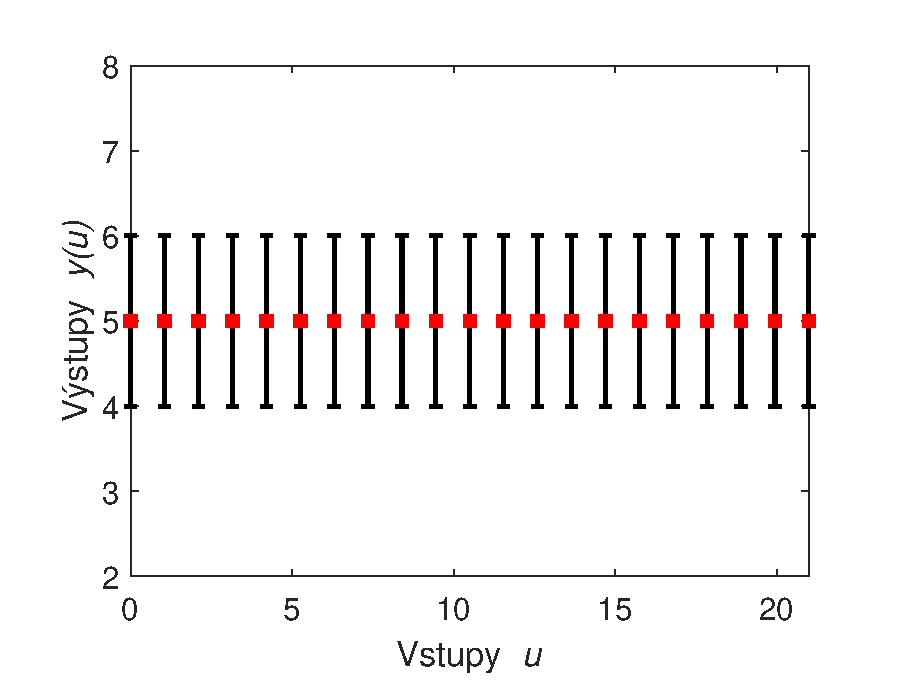
\includegraphics[width=\linewidth]{images/gpe_ex_data1}
		\caption{Namerané výstupné údaje z neznámeho procesu.}
		\label{fig:gpe_ex1_data}
	\end{subfigure}
	\begin{subfigure}[b]{0.48\textwidth}
		\centering
		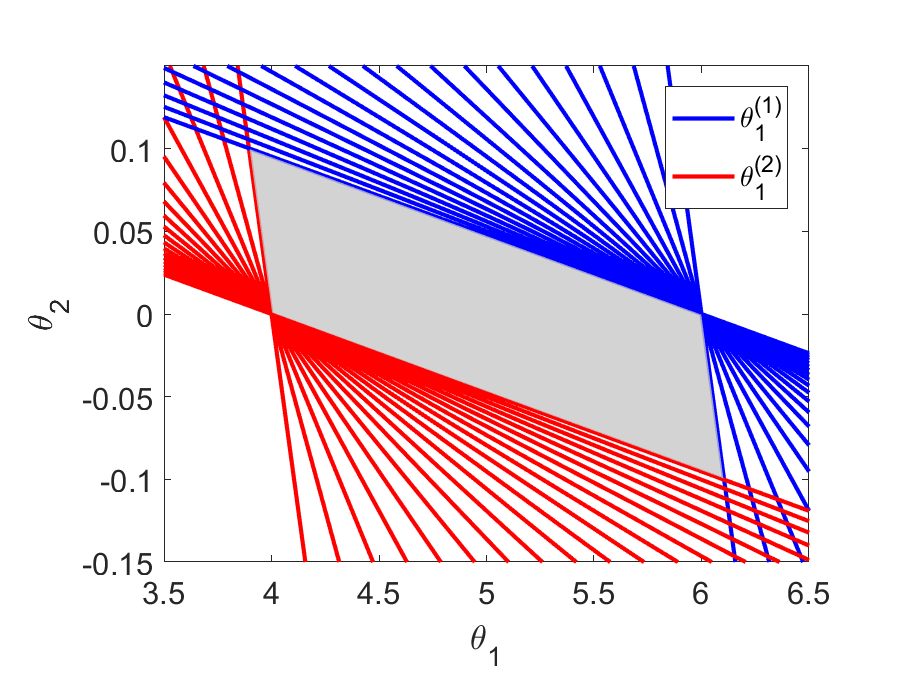
\includegraphics[width=\linewidth]{images/gpe_ex_line1}
		\caption{Grafická metóda garantovaného odhadu parametrov.}
		\label{fig:gpe_ex1_gm}
	\end{subfigure}
	\caption{Ilustračný príklad garantovaného odhadu parametrov --- variant 1 --- zidealizovaný prípad.}
	\label{fig:gpe_ex1}
\end{figure}

Takto sme získali nielen informácie o parametroch nášho modelu, ale aj informácie o zložitosti resp. jednoduchosti štruktúry modelu. Na Obr. \ref{fig:gpe_ex1_gm} vidíme, že parameter $ \theta_2 $ obsahuje vo svojom intervale nulu, čím sa porušuje invariantnosť štruktúry modelu a môžeme tvrdiť, že takýto matematický opis je potenciálne zbytočne zložitý. Rovnaké dáta by sme teda vedeli opísať aj konštantným modelom, t.j. 
\begin{equation}
	\hat{y}(u) = \theta_1.
\end{equation}

 Avšak dáta zobrazené na Obr. \ref{fig:gpe_ex1} boli trošku zidealizované a pravdepodobne v bežnom živote by nenastala situácia, že by senzor niekoľkokrát po sebe nameral tú istú hodnotu. Pozrime sa však, čo sa stane, ak naše namerané údaje budú mať bližšie k realite, tak ako je uvedené na Obr. \ref{fig:gpe_ex2_data}. Ako si môžeme všimnúť na Obr. \ref{fig:gpe_ex2_gm}, odhadované ohraničenie jednotlivých parametrov $ \theta_1, \theta_2 $ sa nám výrazne zmenšilo. Takže môžeme tvrdiť, že samotný šum merania nám prispieva k presnosti odhadu parametrov. 

\begin{figure}
	\centering
	\begin{subfigure}[b]{0.48\textwidth}
		\centering
		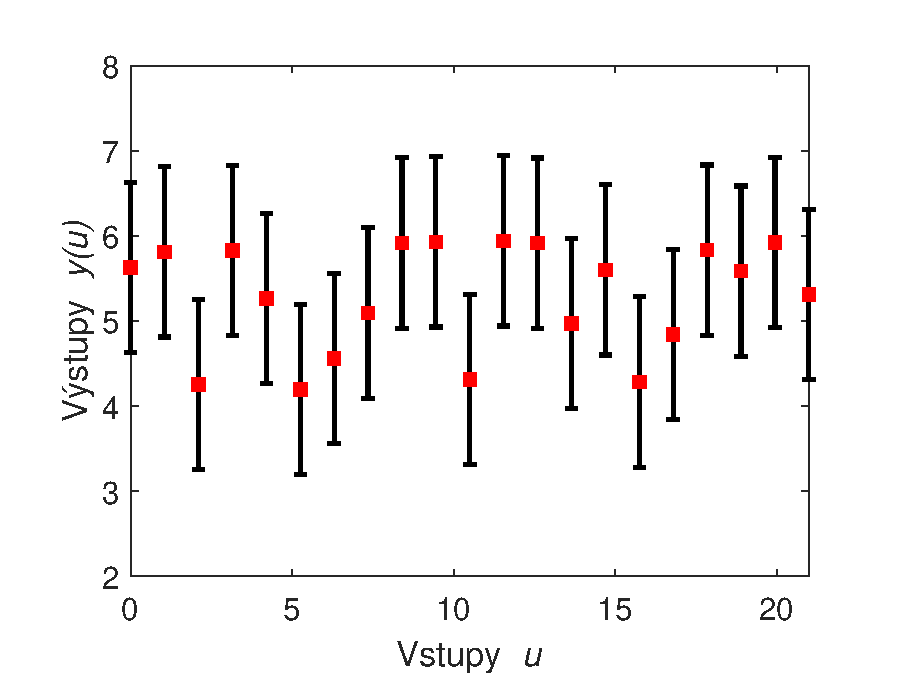
\includegraphics[width=\linewidth]{images/gpe_ex_data2}
		\caption{Namerané výstupné údaje z neznámeho procesu.}
		\label{fig:gpe_ex2_data}
	\end{subfigure}
	\begin{subfigure}[b]{0.48\textwidth}
		\centering
		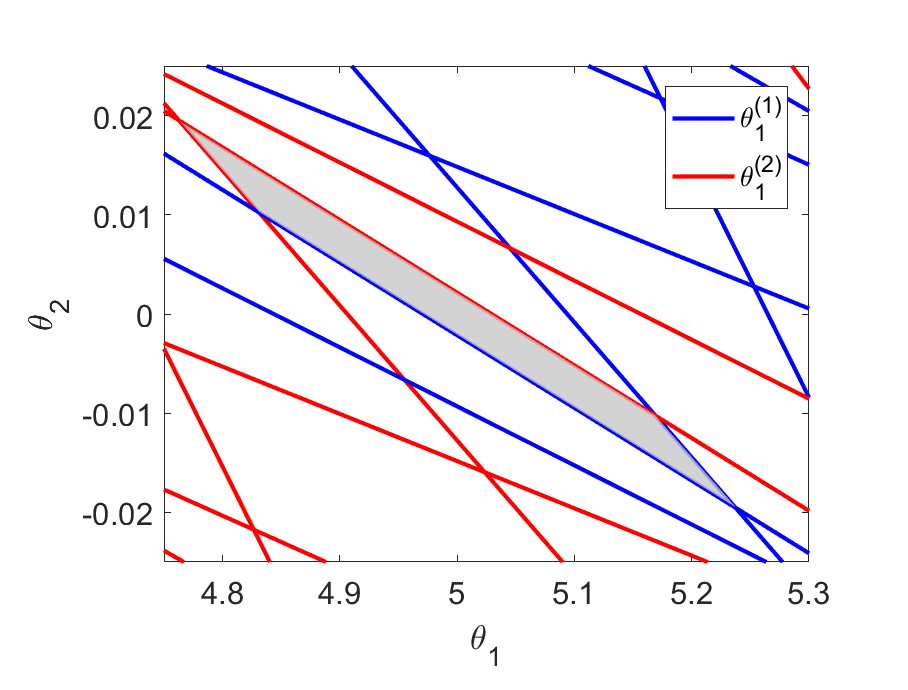
\includegraphics[width=\linewidth]{images/gpe_ex_line2}
		\caption{Grafická metóda garantovaného odhadu parametrov.}
		\label{fig:gpe_ex2_gm}
	\end{subfigure}
	\caption{Ilustračný príklad garantovaného odhadu parametrov --- variant 2.}
	\label{fig:gpe_ex2}
\end{figure}

\section{Mnohorozmerový prípad}
Grafická metóda GOP je krásny ilustračný príklad toho ako táto metóda funguje. Problémom však ostáva, že ak by sme potrebovali odhadovať viac parametrov ako 3 (pri bežných regresných analýzach dátových modelov potrebujeme odhadovať desiatky, možno až stovky parametrov), narážame na obmedzenia tejto metódy --- problém s vizualizáciou. Preto je nutné túto grafickú metódu vymeniť za niečo iné, čo bude obchádzať problematiku s vizualizáciou. Schodnou cestou je transformovať úlohu GOP na optimalizačnú problematiku~\cite{artzova:gpe_moving_hor:2019}, ktorý by mohla vyzerať nasledovne 
\begin{equation}
	\begin{split}
		\left[ \ubar{\theta}_i, \bar{\theta}_i \right] = \min_{\theta} / &\max_{\theta} \quad \theta_i, \quad\qquad \forall i = 1,2, \dots n_\theta, \\
		\text{s.t.}& \quad \ubar{e} \leq y - \hat{y}\left(\theta\right) \leq \bar{e}	
	\end{split}
	\label{eq:gpe:general_form}
\end{equation} 
kde 
\begin{equation*}
	\theta = 
	\begin{pmatrix}
		\ubar{\theta}_1 & \bar{\theta}_1 \\
		\ubar{\theta}_2 & \bar{\theta}_2 \\
		\vdots & \vdots \\
		\ubar{\theta}_{n_\theta} & \bar{\theta}_{n_\theta}	
	\end{pmatrix}.
\end{equation*}

Takto hľadáme minimálnu $ \ubar{\theta}_i $ resp. maximálnu $ \bar{\theta}_i $ hodnotu všetkých 
$ n_\theta $ odhadovaných  parametrov, ktoré nám zaručia, že rozdiel výstupov nameraných $ y $ a modelových $ \hat{y} $ bude ležať v hraniciach chyby merania $ \langle \ubar{e}, \bar{e} \rangle $.

\section{Odhad rádu modelu}
V predchádzajúcej časti sme ukázali ako získať intervalové hodnoty parametrov pre ľubovoľný počet odhadovaných parametrov. Čo sme však zamlčali bolo, že nie každá štruktúra modelu dokáže splniť podmienku optimalizačnej úlohy \eqref{eq:gpe:general_form}. Preto, skôr ako začneme riešiť úlohu odhadu parametrov, potrebujeme odhadnúť vhodnú štruktúru resp. rád modelu. V tejto časti uvedieme ako riešiť problematiku odhadu minimálneho rádu modelu. Úlohu hľadania adekvátneho maximálneho rádu modelu objasníme v časti \aps{Verifikácia dátových modelov}.

Ak nájdeme najjednoduchšiu štruktúru dátového modelu, ktorá vyhovuje optimalizačnej úlohe definovanej v nasledujúcom tvare
\begin{equation}
	\begin{split}
		\min_{\theta} & \quad 0, \\
		\text{s.t} & \quad \ubar{e} \leq y - \hat{y}\left(\theta\right) \leq \bar{e}
	\end{split}
	\label{eq:GPE_m_order_est}
\end{equation}
potom sme našli minimálny rád modelu. $ \theta^T = (\theta_1, \theta_2, \dots, \theta_{n_\theta}) $ je vektor odhadovaných parametrov a $ n_\theta $ predstavuje odhadovaný minimálny rád modelu. Takáto formulácia rieši problematiku prípustnosti, ktorej cieľom je nájsť najjednoduchšiu štruktúru dátového modelu, pri ľubovoľných hodnotách parametrov $ \theta $, ktorá neporušuje ohraničenia optimalizačného problému.  

\section{Verifikácia dátových modelov}
Úlohou verifikácie dátových modelov je overiť správnosť a posúdiť kvalitu daného dátového modelu spomedzi viacerých možností. Existuje množstvo metód a prístupov, ktoré sa snažia riešiť danú problematiku. My spomedzi nich spomenieme tzv. štandardné kritéria a zobrazenie Pareto front.

\subsection{Štandardné kritéria}
Pre štandardné kritéria je základným elementom výberu vhodného modelu zložitosť modelu. Tieto kritéria penalizujú pravdepodobnosť na základe počtu parametrov resp. rádu modelu a veľkosti vzorky. Akaike, v roku 1974, navrhol použitie Kullback–Leibler informačnej hodnoty na výber modelov, ktorým sa ustanovil vzťah medzi informovanosťou, pravdepodobnosťou a Kullback–Leibler maximom. Až neskôr, keď sa stanovil vzťah na odhad  Kullback–Leibler informačnej hodnoty, ju začali nazývať \aps{Akaike information criterion (AIC)} alebo Akaikeho informačné kritérium~\cite{emiliano:stand_crit:2014}. 

Postupom času pribúdali ďalšie informačné kritéria, ktoré nejakým spôsobom modifikovali AIC. Medzi ne patria AIC s korekciou, ktoré sa zvykne označovať ako \aps{AICc} a taktiež Bayesovské informačné kritérium \aps{BIC}. Pri aplikácii týchto kritérií na sadu požadovaných modelov, najlepším modelom je ten, ktorý má najnižšiu hodnotu AIC, AICc alebo BIC.

\subsubsection*{AIC}
Toto kritérium je založené na koncepte informácie a poskytuje relatívnu mieru stratených informácií, keď sa konkrétny model používa na opis skutočného javu~\cite{emiliano:stand_crit:2014}. Akaikeho kritérium možno vyjadriť nasledovne
\begin{equation}
	\text{AIC} = 2k - 2\ln\left( \hat{L} \right),
\end{equation}
kde $ k $ reprezentuje počet parametrov modelu a $ \hat{L} $ je pravdepodobnostná funkcia, ktorá vyjadruje mieru správnosti regresie dát daným modelom. Jednou z takýchto funkcií je aj funkcia hustoty pravdepodobnosti normálneho rozdelenia, ktorej tvar je 
\begin{equation}
	\hat{L} = \prod_i^N \frac{1}{\sigma \sqrt{2\pi}}e^{-\frac{1}{2}\left( \frac{y_i - \hat y_i}{\sigma} \right)^2},
\end{equation}
kde $ \sigma $ je jeho štandardná odchýlka a rozptyl sa označuje ako $ \sigma^2 $.

\subsubsection*{AICc}
Nevýhodou AIC je, že môže nepresne vyhodnotiť kvalitu modelu v prípade, že počet parametrov je väčší ako veľkosť vzorky~\cite{emiliano:stand_crit:2014}. Vtedy je nutné upraviť dané kritérium
\begin{equation}
	\text{AICc} = \text{AIC} + \frac{2k^2 + 2k}{N - k - 1}, 
\end{equation}
kde $ N $ predstavuje veľkosť vzorky dát. AICc by sa malo používať, ak pomer $ \frac{n}{k} $ je malý, napríklad $ \frac{N}{k} < 40$~\cite{kenneth:understanding_stand_crit:2004}. V opačnom prípade, keď je tento pomer dostatočne veľký, obe informačné kritéria by mali vracať podobné výsledky.

\subsubsection*{BIC}
Bayesovské informačné kritérium slúži na hodnotenie kvality modelu, ktoré je založené na posteriornej pravdepodobnosti porovnávaných modelov~\cite{emiliano:stand_crit:2014} a definujú dané informačné kritérium ako
\begin{equation}
	\text{BIC} = \ln\left( N \right)k - 2\ln\left( \hat{L} \right).
\end{equation}

\subsection{Pareto front}
Táto metóda je pomenovaná po talianskom inžinierovi, sociológovi, ekonómovi, politickom vedcovi a filozofovi Vilfredovi Paretovi. On si ako prvý uvedomil, že veľa ekonomických riešení pomáhajú určitej skupine ľudí, zatiaľ čo inej ubližujú. Jeho prácou sa snažil nájsť také riešenie, ktoré  by na jednej strane pomáhalo a na druhej neubližovalo~\cite{mornati:pareto_opt:2013}. 

Problematiku, ktorú riešil Pareto, bola viacúčelová optimalizácia. Pri tomto druhu optimalizácie, kedy rôzne účely (účelové funkcie) sú si odporujúce, najlepšie riešenie nájdeme ako kompromis, pretože nie je možné spraviť zlepšenie v jednom smere bez toho, aby nedošlo k degradácii ostatných. Súbor všetkých Pareto-optimálnych riešení sa nazýva Pareto front, pretože zvyčajne graficky tvorí zreteľný front bodov.

Jednu ukážku Pareto frontu môžeme vidieť na Obr. \ref{fig:Pareto_example}. Modrou sú zobrazené možné optimálne riešenia a červená predstavuje utopický bod -- tento nie je možné nikdy dosiahnuť a predstavuje to najlepšie možné riešenie. Ako sa čítajú takéto grafy? V prvom rade je nutné si uvedomiť, ako sú kvantifikované dané vlastnosti A, B. Povedzme, že väčšia hodnota znamená zhoršenie danej vlastnosti. Ako sa tak pohybujeme po horizontálnej osi, zlepšujeme vlastnosť A, ale pritom zhoršujeme vlastnosť B. Mohli by sme povedať, že bod, ktorý je najbližšie k utopickému bodu, bude predstavovať najlepší možný kompromis medzi oboma vlastnosťami. Takýto predpoklad je správny, ale veľa závisí od profilu frontu. Na Pareto front sa môžeme pozerať ešte inak. Rozdeľme front na dve časti v bode, kde sa výraznejšie mení sklon frontu, napr. keď vlastnosť B dosahuje hodnotu 1. Do tohto bodu, každé výraznejšie zlepšenie vo vlastnosti A, predstavuje menšiu degradáciu vlastnosti B, čo je pre nás výhodnejšie. Avšak, od tohto bodu sa sklon frontu mení a ďalším zlepšovaním vlastnosti A, ktoré by bolo v tom prípade omnoho menšie, by sme výraznejšie zhoršovali vlastnosť B a to by bolo kontraproduktívne.
\begin{figure}
	\centering
	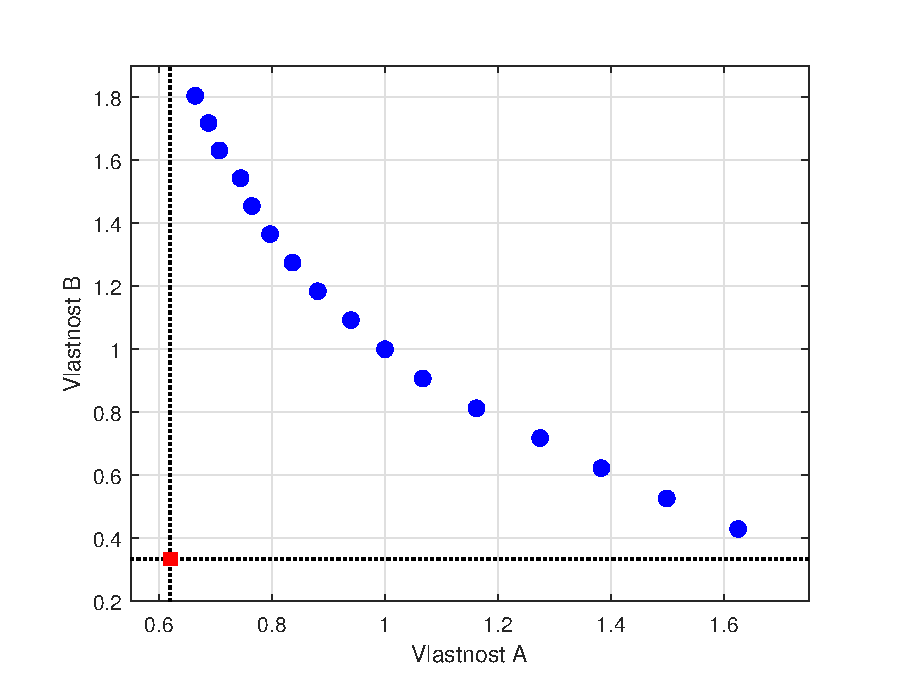
\includegraphics[width=0.7\linewidth]{images/Pareto_ex}
	\caption{Zobrazenie Pareto front -- optimálne riešenia (modrá), utopický bod (červená).}
	\label{fig:Pareto_example}
\end{figure}

Pareto front môžeme využiť aj pri verifikácii kvality dátových modelov. Stačí ak zobrazíme niektoré skúmané vlastnosti vybraného súboru modelov, napríklad trénovacia vs. predikčná kvalita modelu, ktoré sa snažíme zlepšiť, optimalizovať. A na základe predchádzajúcej úvahy vyberieme taký model, ktorý bude predstavovať ten najlepší možný kompromis medzi oboma vlastnosťami. 